
\documentclass[11pt]{article}
\usepackage{amsmath,amssymb}
\usepackage{graphicx}
\usepackage[margin=0.75in]{geometry}
\usepackage{bm}
\usepackage{color}
\usepackage[usenames,dvipsnames]{xcolor}
\usepackage{enumerate}
\usepackage{courier}
\usepackage{float}
\usepackage{verbatim}

\setlength\parindent{0pt}
\newcommand{\pr}{P} % Generic probability
\newcommand{\var}{\textrm{Var}}
\newcommand{\cov}{\textrm{Cov}}


\title{STAT 240 Homework 4}
\author{Rebecca Barter, Andrew Do, and Kellie Ottoboni}
\date{May 1, 2015} % delete this line to display the current date

%%% BEGIN DOCUMENT
\begin{document}

\maketitle


\section*{Problem (1)}
We completed the code in file \texttt{hw4\_functions.R}.  For the dataset 
$$X: -1.0, 1.7, -2.0, 0.6, 0.9, 3.5, \qquad Y : 1.9, -0.3, 2.8, -0.7, 1.6, -2.4$$

we obtained the following p-values setting $\texttt{L}$ to 1,000,000.
\begin{table}[htdp]
\begin{center}
\begin{tabular}{|c|c|c|c|c|}
\hline
 & z Statistic & Wilcoxon Rank Sum & Paired z & Signed Rank  \\ \hline
Normal Approximation & 0.4505772 & 0.5319069 & 0.4625569 & 0.5   \\
Permutation & 0.454514 & 0.531657 & 0.455443 & 0.499427  \\ \hline
\end{tabular}
\end{center}
\label{default}
\end{table}%
 The exact p-value for the sign test was $0.65625$.  Next, we use the dataset 
$$X: 0.5, 2.4, -4.1, 5.9, 3.7, 3.6, \qquad Y : 2.7, 0.8, 1.6, 5.7, 4.3, 0.3$$

We obtained the following p-values setting $\texttt{L}$ to 1,000,000.
\begin{table}[htdp]
\begin{center}
\begin{tabular}{|c|c|c|c|c|}
\hline
 & z Statistic & Wilcoxon Rank Sum & Paired z & Signed Rank  \\ \hline
Normal Approximation & 0.6393479 & 0.5319069 & 0.6826982 & 0.6625066   \\
Permutation & 0.626417 &  0.531804 & 0.626229 & 0.655774  \\ \hline
\end{tabular}
\end{center}
\label{default}
\end{table}%

The p-value for the sign test was $ 0.65625$.

\newpage
\section*{Problem (2)}
We estimated the power (where the alternative hypothesis is $H_1: X > Y$) for each of the five tests from part (1) by generating 100,000 datasets (where $X$ and $Y$ each have sample size 50) according to the specified distribution, and identifying the fraction of null hypotheses rejected at the 0.05 significance level using the normal approximation (except for the sign test). The results are presented in Figure \ref{fig:part2} and Table \ref{tab:part2}.


\begin{figure}[H]
\centering
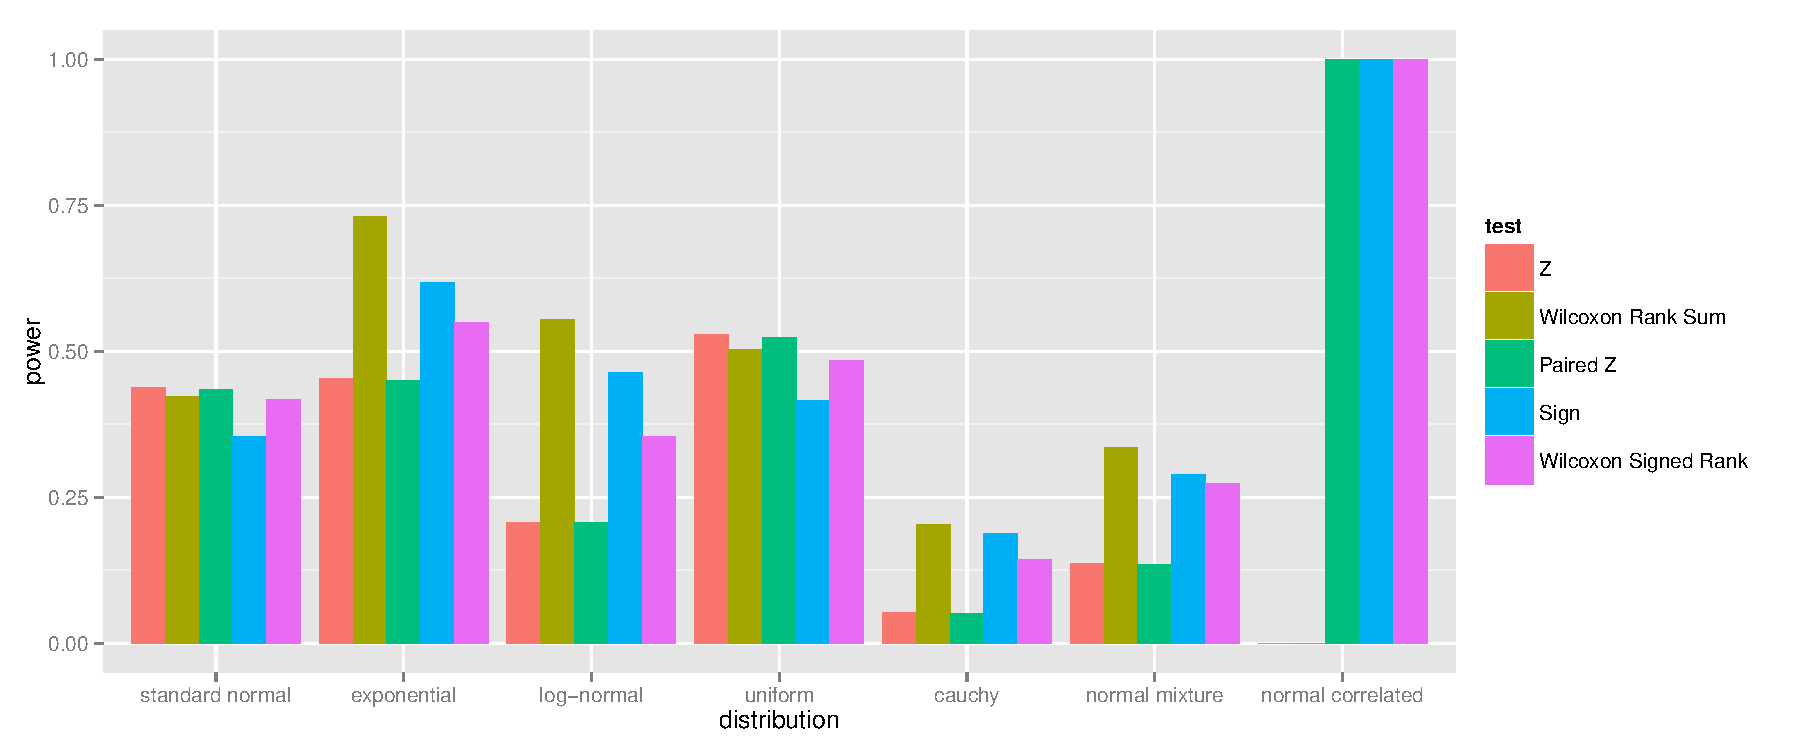
\includegraphics[scale = 0.6]{part2.pdf}
\caption{The power of each test where $Y$ has each of the stated distributions and $X$ has the same distribution as $Y$, but is shifted up by 0.3.}
\label{fig:part2}
\end{figure}


\begin{table}[ht]
\centering
\begin{tabular}{lrrrrrrr}
  \hline
test & std normal & exp & log-normal & uniform & cauchy & normal mix & normal corr \\ 
  \hline
Z & 0.44 & 0.45 & 0.21 & 0.53 & 0.05 & 0.14 & 0.00 \\ 
 Wilcoxon Rank Sum & 0.43 & 0.73 & 0.55 & 0.50 & 0.20 & 0.33 & 0.00 \\ 
 Paired Z & 0.44 & 0.45 & 0.21 & 0.52 & 0.05 & 0.13 & 1.00 \\ 
  Sign & 0.36 & 0.62 & 0.46 & 0.42 & 0.19 & 0.29 & 1.00 \\ 
  Wilcoxon Signed Rank & 0.42 & 0.55 & 0.35 & 0.49 & 0.14 & 0.27 & 1.00 \\ 
   \hline
\end{tabular}
\caption{The power of each test where $Y$ has each of the stated distributions and $X$ has the same distribution as $Y$, but is shifted up by 0.3.}
\label{tab:part2}
\end{table}

\noindent We find that when the data has a standard normal distribution, the tests all have similar power (and surprisingly low power, with the highest power attained being 0.44), with the exception of the sign test which has lower power.\\
 When the data has an exponential distribution, the $Z$ and paired $Z$ tests have the lowest power, but perform similarly to one another. Interestingly, the sign test is a bit more powerful than the Wilcoxon signed rank test, but the Wilcoxon rank sum test is by far superior to the others in terms of power. \\
 When the data follows a log-normal distribution, we find the same results as we did for exponentially distributed data, but the tests are overall less powerful for log-normal data.\\
  When the data has a uniform distribution, the highest power achieved is 0.53, but all tests have similar power except for the sign test which has slightly lower power (0.42).\\ 
  For the Cauchy distribution, the $Z$ and paired $Z$ tests have almost no power (0.05), and the remaining tests have power between 0.14 and 0.20, which is also very low. \\
  For the normal mixture data, the non-parametric methods have much higher power than the parametric methods, but the highest power is still fairly low at 0.33.\\
  Finally, for the example where $X$ and $Y$ are correlated and normal, the unpaired tests (the $Z$ and Wilcoxon rank sum tests) have 0 power, whereas the paired tests (the paired $Z$, sign and Wilcoxon signed rank tests) have power 1.

\newpage
\section*{Problem (3)}
We estimated the power (where the alternative hypothesis is $H_1: X > Y$) for each of the five tests from part (2) by generating 100,000 datasets (where $X$ and $Y$ each have sample size 50) according to the Cauchy distribution once with a shift of 0.5 and once without, and identifying the fraction of null hypotheses rejected at the 0.05 significance level using the normal approximation (except for the sign test). We simulated the same distributions another 10,000 times to estimate the power of the tests but this time using 1,000 permutations of the data to obtain an estimate of the true null.  The results are presented in Figure \ref{fig:part3} and Table \ref{tab:part3}.

\begin{figure}[H]
	\centering
	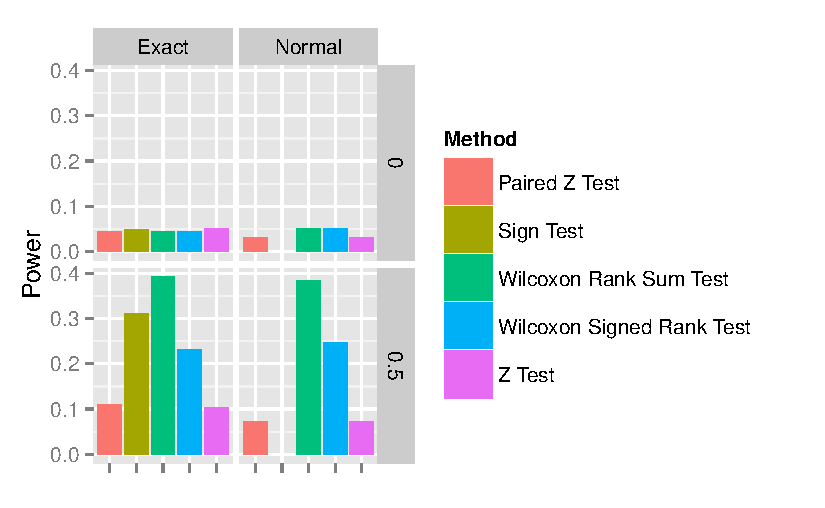
\includegraphics[scale = 1]{part3.pdf}
	\caption{The power of the tests when the true distribution is Cauchy.}
	\label{fig:part3}
\end{figure}

\begin{table}[ht]
	\centering
	\begin{tabular}{rllrr}
		\hline
		& Method & Calculation & Shift & Power \\ 
		\hline
		1 & Z Test & Normal & 0.50 & 0.07 \\ 
		2 & Wilcoxon Rank Sum Test & Normal & 0.50 & 0.38 \\ 
		3 & Paired Z Test & Normal & 0.50 & 0.07 \\ 
		4 & Wilcoxon Signed Rank Test & Normal & 0.50 & 0.25 \\ 
		5 & Z Test & Normal & 0.00 & 0.03 \\ 
		6 & Wilcoxon Rank Sum Test & Normal & 0.00 & 0.05 \\ 
		7 & Paired Z Test & Normal & 0.00 & 0.03 \\ 
		8 & Wilcoxon Signed Rank Test & Normal & 0.00 & 0.05 \\ 
		9 & Z Test & Exact & 0.50 & 0.10 \\ 
		10 & Wilcoxon Rank Sum Test & Exact & 0.50 & 0.39 \\ 
		11 & Paired Z Test & Exact & 0.50 & 0.11 \\ 
		12 & Sign Test & Exact & 0.50 & 0.31 \\ 
		13 & Wilcoxon Signed Rank Test & Exact & 0.50 & 0.23 \\ 
		14 & Z Test & Exact & 0.00 & 0.05 \\ 
		15 & Wilcoxon Rank Sum Test & Exact & 0.00 & 0.04 \\ 
		16 & Paired Z Test & Exact & 0.00 & 0.04 \\ 
		17 & Sign Test & Exact & 0.00 & 0.05 \\ 
		18 & Wilcoxon Signed Rank Test & Exact & 0.00 & 0.04 \\ 
		\hline
	\end{tabular}
	\caption{The power of the tests when the true distribution is Cauchy.}
	\label{tab:part3}
\end{table}

Again we see for the normal approximation, the Z and paired Z tests fair worse in terms of power than their WRS, Sign, and WSR counterparts.  This makes sense because both the Z and paired Z-tests rely on a variance estimate of the true distribution.  The Cauchy distribution has an undefined variance (or "infinite variance"), which throws the Z-statistic off.  Perhaps more fundamental to why these tests fair more poorly on the Cauchy distribution is the fact that our hypotheses are statements about the means of the distribution, which is again, undefined.  The WRS, Sign, and WSR Tests in some sense circumvents this a little by checking for a "modal difference," but we think the fundamental problem remains.  Using a permutations to generate the null distribution gives these tests a little bit more power since the Cauchy distribution does not converge to a normal distribution.
\end{document}